\begin{SCn}
	
\scnsectionheader{\currentname}
	
\scnstartsubstruct
	
\scnheader{Предметная область искусственных нейронных сетей}
\scnidtf{Предметная область и.н.с.}
\scniselement{предметная область}
\scnsdmainclass{искусственная нейронная сеть;действие с искусственной нейронной сетью}
\scnsdclass{искусственная нейронная сеть, }
\scnsdrelation{}

\scnrelfromset{частная предметная область}{
Предметная область обучения искусственных нейронных сетей\\
;Предметная область задач, решаемых с помощью искусственных нейронных сетей\\
}


%\scnrelfromset{частная предметная область}{
%Предметная область ИНС с заданным направлением связей\\
%    \scnaddlevel{1}
%    \scnrelfromset{частная предметная область}{
%    Предметная область ИНС с прямым связями\\
%        \scnaddlevel{1}
%        \scnrelfromset{частная предметная область}{
%        Предметная область персептронов\\
%            \scnaddlevel{1}
%            \scnrelfromset{частная предметная область}{
%            Предметная область персептронов Розенблатта
%            ;Предметная область персептронов Румельхарта
%            ;Предметная область автоэнкодерных ИНС
%            }
%            \scnaddlevel{-1}
%        ;Предметная область ИНС радиально-базисных функций
%        ;Предметная область машин опорных векторов
%        }
%        \scnaddlevel{-1}
%    ;Предметная область ИНС с обратными связями\\
%        \scnaddlevel{1}
%        \scnidtf{Предметная область рекуррентных ИНС}
%        \scnrelfromset{частная предметная область}{
%        Предметная область ИНС Джордана
%        ;Предметная область ИНС Элмана
%        ;Предметная область LSTM-элементов
%        ;Предметная область GRU-элементов
%        }
%        \scnaddlevel{-1}
%    }
%    \scnaddlevel{-1}
%;Предметная область обучения ИНС\\
%    \scnaddlevel{1}
%    \scnrelfromset{частная предметная область}{
%    Предметная область ИНС, обучающихся с учителем
%    ;Предметная область ИНС, обучающихся без учителя\\
%        \scnaddlevel{1}
%        \scnrelfromset{частная предметная область}{
%        Предметная область обучающихся автоэнкодерных ИНС
%        ;Предметная область ИНС глубокого доверия
%        ;Предметная область генеративно-состязательных ИНС
%        ;Предметная область самоорганизующихся карт Кохонена
%        ;Предметная область ИНС Хопфилда
%        ;Предметная область подкрепляющего обучения ИНС
%        }
%        \scnaddlevel{-1}
%    }
%    \scnaddlevel{-1}
%;Предметная область топологий ИНC\\
%    \scnaddlevel{1}
%    \scnrelfromset{частная предметная область}{
%    Предметная область полносвязных ИНC
%    ;Предметная область многослойных ИНC
%    ;Предметная область слабосвязных ИНC
%    }
%    \scnaddlevel{-1}
%;Предметная область задач, решаемых с помощью ИНС\\
%    \scnaddlevel{1}
%    \scnrelfromset{частная предметная область}{
%    Предметная область ИНС, решающих задачу классификации
%    ;Предметная область ИНС, решающих задачу аппроксимации
%    ;Предметная область ИНС, решающих задачу управления
%    ;Предметная область ИНС, решающих задачу фильтрации
%    ;Предметная область ИНС, решающих задачу детекции
%    ;Предметная область ИНС, решающих задачу с ассоциативной памятью
%    }
%    \scnaddlevel{-1}
%;Предметная область интеграции ИНС с базой знаний
%}

\scnheader{искусственная нейронная сеть}
    \scnidtf{и.н.с.}
    \scnidtf{множество искусственных нейронных сетей}
    \scnidtf{нейронная сеть}
    \scnexplanation{
        \textbf{\textit{Искусственная нейронная сеть}} -- это совокупность нейронных элементов и связей между.(TODO:Ссылка на Головко).

        Искусственная нейронная сеть состоит из \textbf{\textit{нейронов}}. Нейроны связанны между собой посредством
        \textbf{\textit{синапсов}}. Нейроны организованы в \textbf{\textit{слои}}. Каждый нейрон слоя принимает сигналы
        со входящих в него синапсов, обрабатывает их единым образом с помощью заданной ему или всему слою
        \textbf{\textit{функции активации}} и передает результат на выходящие из него синапсы.
    }
    \scnexplanation{
        \textbf{\textit{Искусственная нейронная сеть}} - это биологически инспирированная математическая модель,
        обладающая обобщающей способностью после выполнения процедуры обучения. Под обобщающей способностью понимается способность
        модели выдавать корректные результаты для экземпляров, не входящих в обучающую выборку.
    }
    \scnsubset{математическая модель}
    \scnaddlevel{1}
        \scnexplanation{\textbf{\textit{математическая модель}} - это упрощенное описание объекта реального мира, выраженное с помощью математической символики}
    \scnaddlevel{-1}

    \scnrelfrom{изображение}{
        \scnfileimage{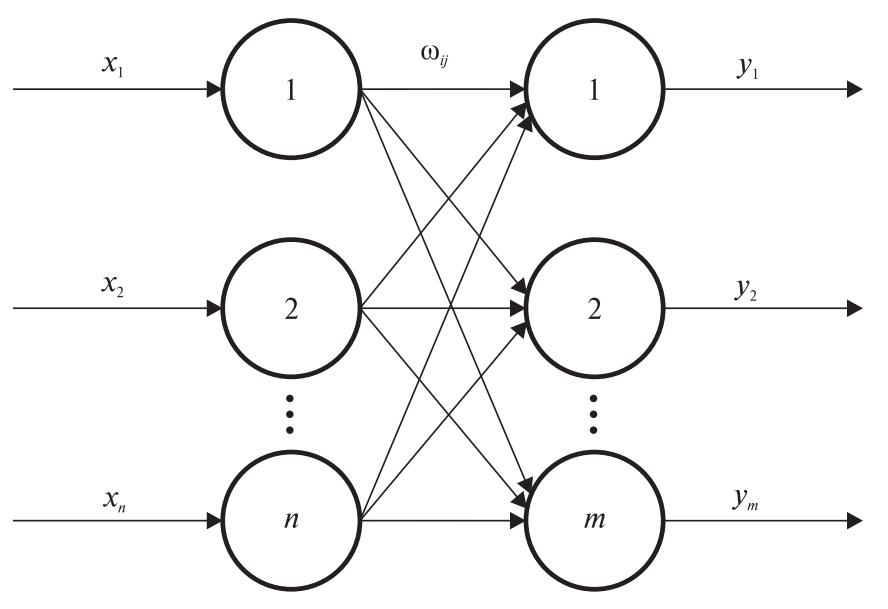
\includegraphics[width=0.4\linewidth]{figures/sd_ps/sd_ann/neural_network.png}}
    }

    \scnrelfrom{описание типичного экземпляра}{
        \scnfilescg{figures/sd_ps/sd_ann/neural_network_scg.png}
    }

    \scnrelfrom{разбиение}{\scnkeyword{Типология и.н.с. по признаку направленности связей\scnsupergroupsign}}
    \scnaddlevel{1}
        \scneqtoset{
        искусственная нейронная сеть с прямыми связями\\
        \scnaddlevel{1}
            \scnsubdividing{
                персептрон\\
                \scnaddlevel{1}
                    \scnsubdividing{
                        персептрон Розенблатта;
                        персептрон Румельхарта;
                        автоэнкодерная искусственная нейронная сеть
                    }
                \scnaddlevel{-1}
                ;машина опорных векторов
                ;искусственная нейронная сеть радиально-базисных функций
            }
        \scnaddlevel{-1}
        ;искусственная нейронная сеть с обратными связями
        \scnaddlevel{1}
            \scnidtf{рекуррентная искусственная нейронная сеть}
            \scnsubdividing{
            искусственная нейронная сеть Джордана
            ;искусственная нейронная сеть Элмана
            ;LSTM-элемент
            ;GRU-элемент
            }
        \scnaddlevel{-1}
        }
    \scnaddlevel{-1}

    \scnrelfrom{разбиение}{\scnkeyword{Типология и.н.с. по признаку полноты связей\scnsupergroupsign}}
    \scnaddlevel{1}
        \scneqtoset{
        полносвязная искусственная нейронная сеть\\
        ;слабосвязная искусственная нейронная сеть
        }
    \scnaddlevel{-1}

    \scnrelfrom{разбиение}{\scnkeyword{Типология и.н.с. по признаку количества слоев\scnsupergroupsign}}
    \scnaddlevel{1}
        \scneqtoset{
        однослойная искусственная нейронная сеть\\
        ;многослойная искусственная нейронная сеть
        }
    \scnaddlevel{-1}

\scnheader{нейрон}
    \scnidtf{искусственный нейрон}
    \scnidtf{множество нейронов искусственных нейронных сетей}
    \scnidtf{математическая модель реального биологического нейрона}
    \scnsubset{искусственная нейронная сеть}
    \scnrelfrom{изображение}{
        \scnfileimage{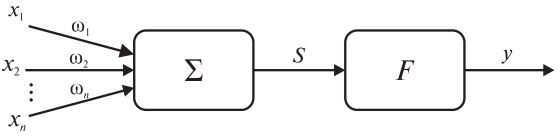
\includegraphics[width=0.4\linewidth]{figures/sd_ps/sd_ann/neuron.png}}
    }
    \scnnote{нейроны могут иметь полный набор связей с нейронами предшествующего слоя или неполный (разряженный)
        набор связей. Сверточный нейрон с соответствующим ему ядром свертки может быть представлен нейроном
        с неполным набором связей}

    \scnsubdividing{
        полносвязный нейрон\\
        \scnaddlevel{1}
            \scnidtf{нейрон, у которого есть полный набор связей с нейронами предшествующего слоя}
            \scnidtf{отдельный обрабатывающий элемент и.н.с., выполняющий функциональное преобразование взвешенной суммы
                компонент вектора входных значений с помощью функции активации}
        \scnaddlevel{-1}
        ;сверточный нейрон\\
        \scnaddlevel{1}
            \scnidtf{отдельный обрабатывающий элемент и.н.с., выполняющий функциональное преобразование результата
                операции свертки матрицы входных значений с помощью функции активации}
        \scnaddlevel{-1}
        ;рекуррентный нейрон\\
        \scnaddlevel{1}
            \scnidtf{нейрон, имеющий обратную связь с самим собой или с другими нейронами и.н.с.}
        \scnaddlevel{-1}
    }

\scnheader{слой}
    \scnidtf{слой и.н.с.}
    \scnidtf{множество слоев искусственных нейронных сетей}
    \scnsubset{искусственная нейронная сеть}
    \scnexplanation{
        \textbf{\textit{Слой и.н.с}}  – это множество нейронных элементов, на которые в каждый такт времени
        параллельно поступает информация от других нейронных элементов сети.TODO: ссылка на Головко
    }
    \scnexplanation{
        \textbf{\textit{слой}} - это множество нейронов, осуществляющих параллельную независимую обработку
        вектора или матрицы входных значений
    }
    \scnnote{функция активации слоя является функцией активации всех нейронов этого слоя}
    \scnnote{конфигурация слоя задается типом, количеством нейронов, функцией активации}
    \scnnote{описание последовательности слоев и.н.с. с конфигурацией каждого слоя задает архитектуру и.н.с.}

    \scnsubdividing{
        полносвязный слой\\
        \scnaddlevel{1}
            \scnidtf{слой, в котором каждый нейрон имеет связь с каждым нейроном предшествующего слоя}
            \scnidtf{слой, в котором каждый нейрон является полносвязным}
        \scnaddlevel{-1}
        ;сверточный слой\\
        \scnaddlevel{1}
            \scnidtf{слой, в котором каждый нейрон является сверточным}
        \scnaddlevel{-1}
        ;слой нелинейного преобразования\\
        \scnaddlevel{1}
            \scnidtf{слой, осуществляющий нелинейное преобразование входных данных}
            \scnexplanation{как правило, выделяются в отдельные слои только в программных реализациях. Фактически
                рассматриваются как финальный этап расчета выходной активности любого нейрона -- применение функции
                активации}
            \scnnote{не изменяет размерность входных данных}
        \scnaddlevel{-1}
        ;dropout слой\\
        \scnaddlevel{1}
            \scnidtf{слой, реализующий технику регуляризации dropout}
            \scnnote{данный тип слоя функционирует только во время обучения и.н.с.}
            \scnexplanation{поскольку полносвязные слои имеют большое количество настраиваемых параметров, они
                подвержены эффекту переобучения. Один из способов устранить такой негативный эффект -- выполнить
                частичный отсев результатов на выходе полносвязного слоя. На этапе обучения техника dropout позволяет
                отбросить выходную активность некоторых нейронов с определенной, заданной вероятностью. Выходная
                активность ``отброшенных'' нейронов полагается равной нулю.}
        \scnaddlevel{-1}
        ;pooling слой\\
        \scnaddlevel{1}
            \scnidtf{подвыборочный слой}
            \scnidtf{объединяющий слой}
            \scnidtf{слой, осуществляющий уменьшение размерности входных данных}
        \scnaddlevel{-1}
        ;слой батч-нормализации\\
    }


\scnheader{экземпляр}
\scnaddlevel{1}
	\scnidtf{instance}
	\scnidtf{пример}
	\scnidtf{example}
	\scnidtf{образ}
	\scnidtf{один объект, наблюдение, транзакция или запись, выраженный в виде вектора или матрицы, компоненты которого представлены численными и/или категориальными значениями}
\scnaddlevel{-1}

\scnheader{признаки}
\scnaddlevel{1}
	\scnidtf{features}
	\scnidtf{входные атрибуты, используемые для предсказания целевой переменной}
	\scnidtf{компоненты вектора или матрицы экземпляра}
	\scnnote{могут быть как численными, так и категориальными}
\scnaddlevel{-1}

\scnheader{обучающая выборка}
\scnaddlevel{1}
	\scnidtf{выборка экземпляров, используемая для изменения параметров н.с. в процессе ее обучения}
	\scnidtf{training set}
\scnaddlevel{-1}

\scnheader{параметры нейронной сети}
\scnaddlevel{1}
\scnidtf{переменные, значения которых изменяются в ходе процедуры обучения}
\scnidtf{компоненты векторов весовых коэффициентов, ядер свертки и пороги нейронов и.н.с.}
\scnaddlevel{-1}

\scnheader{вектор весовых коэффициентов}
\scnaddlevel{1}
	\scnidtf{вектор параметров отдельно взятого нейрона, компоненты которого изменяются в процессе обучения и.н.с.}
\scnaddlevel{-1}

\scnheader{ядро свертки}
\scnaddlevel{1}
	\scnidtf{квадратная матрица произвольной размерности, компоненты которой изменяются в процессе обучения и.н.с.}
\scnaddlevel{-1}

\scnheader{порог нейрона}
\scnaddlevel{1}
	\scnidtf{скаляр, значение которого изменяется в процессе обучения и.н.с.}
\scnaddlevel{-1}

\scnheader{связь}
\scnaddlevel{1}
	\scnidtf{логическое соединение между двумя нейронами, определяющее направление передачи данных и характеризующееся соответствующим компонентом вектора весовых коэффициентов или ядра свертки}
	\scnnote{в случае полносвязного нейрона влияние связи на выходную активность нейрона определяется соответствующим компонентом вектора весовых коэффициентов}
\scnaddlevel{-1}

\scnheader{предшествующий слой}
\scnaddlevel{1}
	\scnidtf{слой, расположенный в последовательности слоев архитектуры и.н.с. ранее рассматриваемого слоя}
\scnaddlevel{-1}

\scnheader{вектор входных значений}
\scnaddlevel{1}
	\scnidtf{вектор экземпляра, компоненты которого прошли предварительную обработку}
	\scnexplanation{такая предварительная обработка как правило включает в себя трансформацию категориальных признаков в численные, а также нормализацию, проектирование признаков, обработку нейронами предшествующих слоев и.н.с. и т.д.}
\scnaddlevel{-1}

\scnheader{матрица входных значений}
\scnaddlevel{1}
	\scnidtf{матрица экземпляра, компоненты которого прошли предварительную обработку}
	\scnexplanation{такая предварительная обработка как правило включает в себя трансформацию категориальных признаков в численные, а также нормализацию, проектирование признаков, обработку нейронами предшествующих слоев и.н.с. и т.д.}
	\scntext{теоретическая неточность}{использование матрицы как формы представления входных данных является серьезным допущением, так как на практике входные данные структурированы более сложно -- в многомерные массивы. Самым близким теоретическим аналогом
 здесь выступает тензор. К сожалению, описание теории нейроных сетей с помощью тензорного исчисления в литературе как таковое отсутствует, но активно используется на практике: например, во многих разрабатываемых нейросетевых фреймворках.
Формализация нейронных сетей с помощью тензоров видится авторам наиболее вероятным направлением работы в ближайших изданиях стандарта OSTIS. }
\scnaddlevel{-1}

\scnheader{взвешенная сумма входных значений}
\scnaddlevel{1}
	\scnidtf{скалярное произведение векторов входных значений и весовых коэффициентов нейрона}
	\scnidtf{взвешенная сумма}
	\scnidtf{в.с.}
	\scnrelfrom{формула}{
		\begin{equation*}
			S = \sum_{i=1}^{n} w_ix_i
		\end{equation*}
		где \textit{n} -- размерность вектора входных значений, $w_i$ -- \textit{i}-тый компонент вектора весовых коэффициентов, $x_i$ -- \textit{i}-тый компонент вектора входных значений
	}
\scnaddlevel{-1}

\scnheader{функция активации нейрона}
\scnaddlevel{1}
	\scnidtf{функция, результат применения которой к в.с. нейрона определяет его выходное значение}
	\scnrelfromvector{виды функций активации}{
		линейная\\
		\scnaddlevel{1}
		\scnrelfrom{формула}{
			\begin{equation*}
				y = kS
			\end{equation*}
			где \textit{k} -- коэффициент наклона прямой, \textit{S} -- в.с.
		}
		\scnaddlevel{-1}
		;пороговая\\
		\scnaddlevel{1}
		\scnrelfrom{формула}{
			\begin{equation*}
				y = sign(S) =
				\begin{cases}
					1, S > 0,\\
					0, S \leq 0
				\end{cases}
			\end{equation*}
		}
		\scnaddlevel{-1}
		;сигмоидная\\
		\scnaddlevel{1}
		\scnrelfrom{формула}{
			\begin{equation*}
				y = \frac{1}{1+e^{-cS}}
			\end{equation*}
			где \textit{с} > 0 -- коэффициент, характеризующий ширину сигмоидной функции по оси абсцисс, \textit{S} -- в.с.
		}
		\scnaddlevel{-1}
		;гиперболический тангенс\\
		\scnaddlevel{1}
		\scnrelfrom{формула}{
			\begin{equation*}
				y = \frac{e^{cS}-e^{-cS}}{e^{cs}+e^{-cS}}
			\end{equation*}
			где \textit{с} > 0 -- коэффициент, характеризующий ширину сигмоидной функции по оси абсцисс, \textit{S} -- в.с.
		}
		\scnaddlevel{-1}
		;softmax\\
		\scnaddlevel{1}
		\scnrelfrom{формула}{
			\begin{equation*}
				y_j = softmax(S_j) = \frac{e^{S_j}}{\sum_{j} e^{S_j}}
			\end{equation*}
			где $S_j$ -- в.с. \textit{j}-го выходного нейрона
		}
		\scnaddlevel{-1}
		;ReLU\\
		\scnaddlevel{1}
		\scnrelfrom{формула}{
			\begin{equation*}
				y = F(S) =
				\begin{cases}
					S, S > 0,\\
					kS, S \leq 0
				\end{cases}
			\end{equation*}
			где \textit{k} = 0 или принимает небольшое значение, например, 0.01 или 0.001.
		}
		\scnaddlevel{-1}
	}
\scnaddlevel{-1}

\scnheader{тестовая выборка}
\scnaddlevel{1}
	\scnidtf{test set}
	\scnidtf{контрольная выборка}
	\scnidtf{выборка экземпляров, используемая для проверки обобщающей способности обученной и.н.с.}
	\scnnote{элементы контрольной выборки не используются в процессе обучения}
\scnaddlevel{-1}

\scnheader{валидационная выборка}
\scnaddlevel{1}
	\scnidtf{выборка экземпляров, используемая для определения (настройки) гиперпараметров и.н.с.}
	\scnnote{элементы валидационной выборки не используются в процессе обучения}
\scnaddlevel{-1}

\scnheader{гиперпараметры и.н.с}
\scnaddlevel{1}
\scnidtf{набор параметров и.н.с., определяющих ее архитектуру (количество слоев и.н.с., количество нейронов в каждом слое и т.д.)}
\scnaddlevel{-1}

\scnheader{обучение}
\scnaddlevel{1}
	\scnidtf{процесс итеративного изменения параметров и.н.с., минимизирующий некоторую заданную функцию потерь, для достижения приемлемого уровня обобщающей способности}
	\scnrelfromvector{основные подходы}{
		обучение с учителем
		\scnaddlevel{1}
			\scnidtf{процесс изменения параметров и.н.с, минимизирующий разницу между выходом и.н.с. и целевой переменной для элементов обучающей выборки, относительно некоторой заданной функции потерь}
		\scnaddlevel{-1}
		;обучение без учителя
		\scnaddlevel{1}
			\scnidtf{процесс изменения параметров и.н.с. без использования заданных целевых переменных (в режиме самоорганизации)}
		\scnaddlevel{-1}
	}
\scnaddlevel{-1}

\scnheader{алгоритм обучения}
\scnaddlevel{1}
   \scnidtf{алгоритм, определяющий процедуру обучения и.н.с. и задающийся правилами изменения параметров и.н.с., а также наборами общих и специальных параметров}
\scnaddlevel{-1}

\scnheader{функция потерь}
\scnaddlevel{1}
	\scnidtf{функция, используемая для вычисления ошибки, рассчитываемой как разница между фактическим эталонным значением и прогнозируемым значением, получаемым и.н.с.}
	\scnrelfromvector{виды функций потерь}{
		MSE\\
		\scnaddlevel{1}
			\scnidtf{mean square error}
			\scnidtf{средняя квадратичная ошибка}
			\scnrelfrom{формула}{
				\begin{equation*}
					MSE = \frac{1}{m} \sum_{i=1}^m (y_i - e_i)^2
				\end{equation*}
				где $y_i$ -- прогноз модели, $e_i$ -- ожидаемый (эталонный) результат, \textit{m} -- размерность выходного вектора
			}
		\scnaddlevel{-1}
		;BCE\\
		\scnaddlevel{1}
			\scnidtf{binary cross entropy}
			\scnidtf{бинарная кросс-энтропия}
			\scnrelfrom{формула}{
				\begin{equation*}
					BCE = -(e \log(y) + (1 - e)\log(1 - y))
				\end{equation*}
				где $y$ -- прогноз модели, $e$ -- ожидаемый (эталонный) результат: \textit{0} или \textit{1}
			}
			\scnnote{для бинарной кросс-энтропии в выходном слое и.н.с. будет находиться один нейрон}
		\scnaddlevel{-1}
		;MCE\\
		\scnaddlevel{1}
			\scnidtf{multi-class cross entropy}
			\scnidtf{мультиклассовая кросс-энтропия}
			\scnrelfrom{формула}{
				\begin{equation*}
					MCE = - \sum_{i=1}^m e_{i} \log(y_{i})
				\end{equation*}
				где $y_{i}$ -- прогноз модели, $e_i$ -- ожидаемый (эталонный результат), \textit{m} -- размерность выходного вектора
			}
			\scnnote{для мультиклассовой кросс-энтропии количество нейронов в выходном слое и.н.с. совпадает с количеством классов}
		\scnaddlevel{-1}
	}
	\scnnote{для решения задачи классификации рекомендуется использовать бинарную или мультиклассовую кросс-энтропийную функцию потерь, для решения задачи регрессии рекомендуется использовать среднюю квадратичную ошибку}
\scnaddlevel{-1}

\scnheader{параметры обучения}
\scnaddlevel{1}
   \scnidtf{группа наиболее общих параметров, которая есть в любом алгоритме обучения и.н.с.}
   \scnrelfromvector{состав группы параметров обучения}{
       скорость обучения\\
          \scnaddlevel{1}
              \scnidtf{параметр, определяющий скорость изменения параметров и.н.с. в процессе обучения}
          \scnaddlevel{-1}
       ;моментный параметр\\
          \scnaddlevel{1}
                \scnidtf{момент}
                \scnidtf{momentum}
                \scnidtf{параметр, используемый в процессе обучения для устранения проблемы ``застревания'' алгоритма обучения в локальных минимумах минимизируемой функции потерь}
                \scnexplanation{при обучении и.н.с. частой является ситуация остановки процесса в определенной точке локального минимума без достижения желаемого уровня обобщающей
                способности и.н.с. Для устранения такого нежелательного явления вводится дополнительный параметр (момент) позволяющий алгоритму обучения ``перескочить'' через
                локальный минимум и продолжить процесс}
         \scnaddlevel{-1}
       ;параметр регуляризации\\
         \scnaddlevel{1}
             \scnidtf{параметр, применяемый для контроля уровня переобучения и.н.с.}
         \scnaddlevel{-1}
       ;размер мини-батча\\
         \scnaddlevel{1}
               \scnidtf{размер группы экземпляров, которая используется для изменения параметров и.н.с. на каждом элементарном шаге обучения}
         \scnaddlevel{-1}
       ;количество эпох обучения
   }
\scnaddlevel{-1}

\scnheader{задачи, решаемые и.н.с.}
\scnaddlevel{1}
	\scnidtf{задачи, которые могут быть решены с помощью и.н.с. с приемлемой точностью}
	\scnrelfromvector{виды задач}{
		классификация экземпляров
			\scnaddlevel{1}
				\scnidtf{задача построения классификатора, т.е. отображения $\tilde c: X \rightarrow C$, где $ X \in \mathbb{R}^m$ -- признаковое пространство экземпляров, $C = {C_1, C_2, ...C_k }$ -- конечное и обычно небольшое множество меток классов.}
			\scnaddlevel{-1}
		;регрессия
			\scnaddlevel{1}
				\scnidtf{задача построения оценочной функции по примерам $(x_i, f(x_i))$, где $f(x)$ -- неизвестная функция}
			\scnaddlevel{-1}
		;кластеризация
			\scnaddlevel{1}
			   \scnidtf{задача разбиения множества экземпляров на группы (кластеры) по какой-либо метрике сходства}
			\scnaddlevel{-1}
		;понижение размерности
			\scnaddlevel{1}
			   \scnidtf{задача уменьшения размерности признакового пространства}
			\scnaddlevel{-1}
	}
\scnaddlevel{-1}

\scnheader{оценочная функция}
\scnaddlevel{1}
	\scnidtf{отображение вида $\tilde{f}: X \rightarrow \mathbb{R}$, где $X \in \mathbb{R}^m$ -- признаковое пространство экземпляров}
\scnaddlevel{-1}

\scnheader{целевая переменная}
\scnaddlevel{1}
	\scnidtf{цель}
	\scnidtf{target}
	\scnidtf{метка}
	\scnidtf{label}
	\scnidtf{численная или категориальная переменная, которая предсказывается для каждого нового экземпляра}
\scnaddlevel{-1}

\scnstartsubstruct
\scnheader{Предметная область обучения искусственных нейронных сетей}
\scnidtf{Предметная область обучения и.н.с.}
\scniselement{предметная область}
\scnsdmainclass{искусственная нейронная сеть, действие обучения искусственных нейронных сетей}
\scnsdclass{}
\scnsdrelation{}
\scnendstruct

\scnstartsubstruct
\scnheader{Предметная область задач, решаемых с помощью искусственных нейронных сетей}
\scnidtf{Предметная область задач, решаемых с помощью и.н.с}
\scniselement{предметная область}
\scnsdmainclass{искусственная нейронная сеть}
\scnsdclass{}
\scnsdrelation{}
\scnendstruct

\scnendsubstruct \scnendcurrentsectioncomment

\end{SCn}